\documentclass{article}[18pt]
\usepackage{../../../../format}
\lhead{CSys}


\begin{document}
\begin{center}
\underline{\huge Circuits}
\end{center}
\section{Key Circuits}
Combinatorial/Combinational Circuits:
\begin{itemize}
	\item \textbf{Adders} - Add the contents of two registers
	\item \textbf{Decoders} - Use a binary number to activate a single line (select one out of many things based on a number of inputs)
	\item \textbf{Multiplexors} - Use a binary number to select an input
\end{itemize}
Sequential circuits:
\begin{itemize}
	\item Latches/flip-flops - basic memory element
\end{itemize}
\section{Half adder}
Based on the simple binary addition rules
\begin{center}
	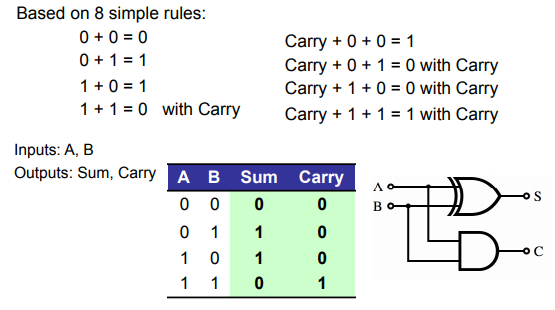
\includegraphics[scale=0.7]{half_adder}
\end{center}

\section{Adder}
Input is not just A and B, but A, B and the carry from the previous bit
Use two half-adders: Add A and B first, then add in the carried bit: 
\begin{center}
	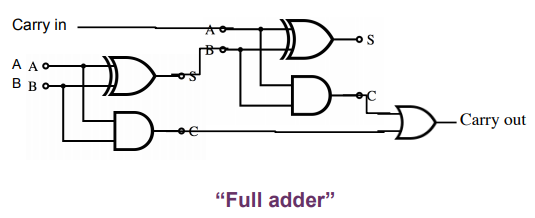
\includegraphics[scale=0.7]{adder}
\end{center}
\section{Chaining adders}
Full adders can be chained to give more bits of input
\begin{center}
	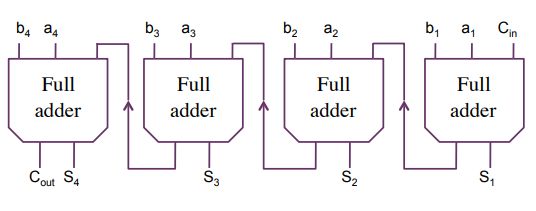
\includegraphics[scale=0.7]{chain_adder}
\end{center}
\section{Subtractor}
Using twos compliment negative we can subtract numbers. Flip each of the bits with a not gate. Set the carry in to 1 in order to add 1
\begin{center}
	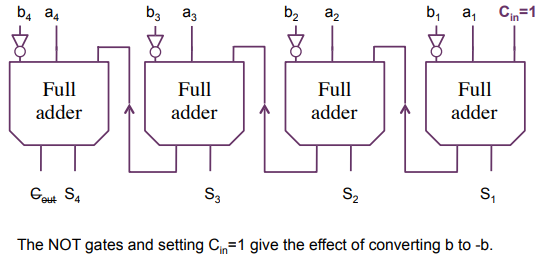
\includegraphics[scale=0.7]{subtractor}
\end{center}
\section{Decoder}
This is used to identify which piece of memory is being talked about when giving an address\\

This is what a decoder does:
\begin{itemize}

\item N inputs. 2N outputs.
\item Only one output is high at a time.
\item Which one depends on the input

\end{itemize}
\begin{center}
	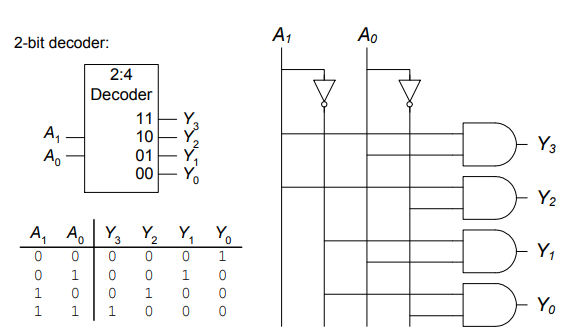
\includegraphics[scale=0.7]{decoder}
\end{center}
Larger decoders require multi-input AND gates to
be construct in two-level logic.\\
This requires a lot of circuitry for large decoders.\\
Can create deeper circuits with fewer transistors,
at the cost of slower response.
\section{Multiplexor}
\begin{center}
	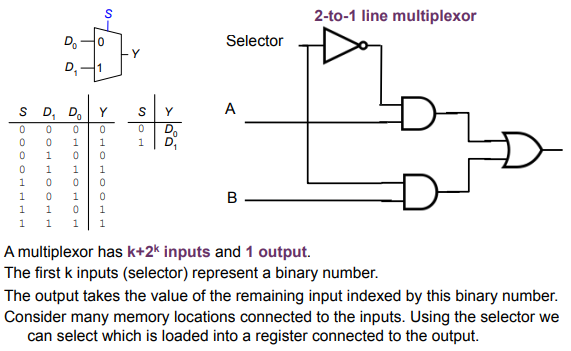
\includegraphics[scale=0.7]{multiplexor}
\end{center}
\begin{itemize}
	\item This allows us to select between data streams
\end{itemize}
\section{Tristate}
\begin{center}
	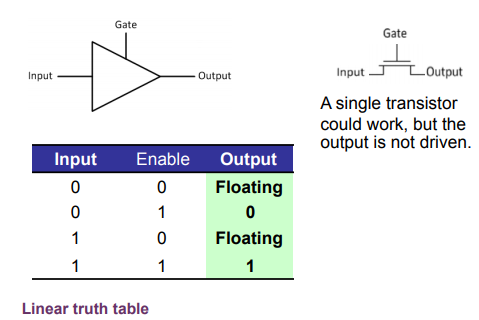
\includegraphics[scale=0.7]{tristate}
\end{center}
\begin{itemize}
	\item Driven low - connected to low voltage line
	\item Driven high - connected to high voltage line
	\item Floating - not connected to anything
	\item This helps when there are weak signals in the circuit
\end{itemize}

\subsection{Inverting Tristate}
\begin{center}
	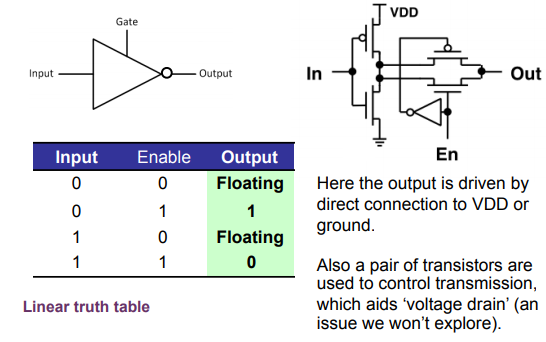
\includegraphics[scale=0.7]{inverting_tristate}
\end{center}
\begin{itemize}
	\item Means the output is driven directly from either the high or low voltage line.
	\item Makes the driven signal strong
	\item When not enabled get floating output
	\item Actual tristate just an inverted inverted tristate
\end{itemize}
\section{Mux}
\begin{center}
	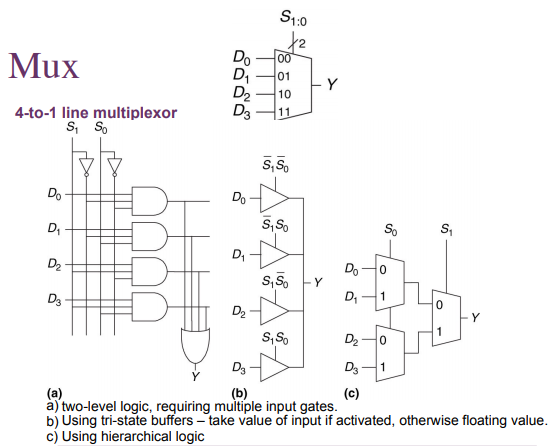
\includegraphics[scale=0.7]{mux}
\end{center}
\begin{itemize}
	\item Using tristate gates a much more efficient multiplexor can be formed
	\item Multiplexors can also be made using hierarchical logic, chaining them together
\end{itemize}
\section{Building a simple ALU}
\begin{center}
	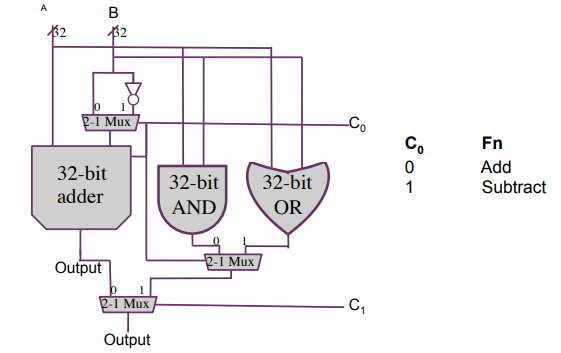
\includegraphics[scale=0.7]{ALU}
\end{center}
\begin{itemize}
	\item The mux is used for the subraction part of the circuit as it can invert the data line
	\item Using the two control bits you can decide between ADD, SUBTRACT, AND, OR. 
\end{itemize}

\end{document}